%% ============================================================
%% f2012_shandong_sci_q16_rolling.tex
%% 2012 山东卷（理科）第 16 题 单位圆沿 x 轴正向滚动
%% 来源 PDF：普通高考/2012/2012山东理.pdf 第 1 页（印面 759）第 3 栏
%% 坐标取自原页矢量层（bp），原点为图区左上角 (890.0,262.0)，y 向下。
%% 第 266.6bp 处 31.4bp 的横线是题面填空横线，不属图稿，已排除。
%% ============================================================
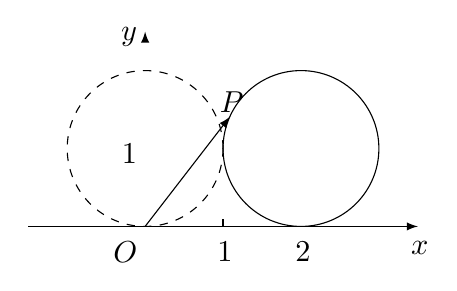
\begin{tikzpicture}[x=1bp,y=-1bp,
  every node/.style={inner sep=0,font=\fontsize{10.5pt}{12.6pt}\selectfont},
  line cap=butt, line join=miter]
  \draw[line width=0.398bp] (3.453,83.676) -- (140.133,83.676);
  \fill[black] (143.719,83.676) .. controls (142.656,83.477) and (140.93,82.879) .. (139.734,82.184) -- (139.734,85.168) .. controls (140.93,84.473) and (142.656,83.875) .. (143.719,83.676);
  \fill[black] (45.535,13.543) .. controls (45.336,14.605) and (44.738,16.332) .. (44.039,17.527) -- (47.027,17.527) .. controls (46.332,16.332) and (45.73,14.605) .. (45.535,13.543);
  \draw[line width=0.398bp] (73.586,83.676) -- (73.586,80.871);
  \draw[line width=0.398bp] (129.691,55.625) .. controls (129.691,40.129) and (117.133,27.57) .. (101.641,27.57) .. controls (86.145,27.57) and (73.586,40.129) .. (73.586,55.625) .. controls (73.586,71.117) and (86.145,83.676) .. (101.641,83.676) .. controls (117.133,83.676) and (129.691,71.117) .. (129.691,55.625) -- cycle;
  \draw[line width=0.398bp] (45.535,83.676) -- (73.816,47.055);
  \fill[black] (76.012,44.215) .. controls (75.203,44.934) and (73.672,45.938) .. (72.391,46.457) -- (74.758,48.285) .. controls (74.938,46.91) and (75.52,45.176) .. (76.012,44.215);
  \draw[line width=0.398bp, dash pattern=on 2.989bp off 2.989bp] (73.586,55.625) .. controls (73.586,40.129) and (61.027,27.57) .. (45.535,27.57) .. controls (30.039,27.57) and (17.48,40.129) .. (17.48,55.625) .. controls (17.48,71.117) and (30.039,83.676) .. (45.535,83.676) .. controls (61.027,83.676) and (73.586,71.117) .. (73.586,55.625) -- cycle;
  \node[anchor=base west] at (36.66,16.82) {$y$};
  \node[anchor=base west] at (72.28,42.56) {$P$};
  \node[anchor=base west] at (36.94,61.06) {$1$};
  \node[anchor=base west] at (141.11,93.96) {$x$};
  \node[anchor=base west] at (71.33,96.21) {$1$};
  \node[anchor=base west] at (99.39,96.21) {$2$};
  \node[anchor=base west] at (33.89,96.61) {$O$};
\end{tikzpicture}
